\twohead{Introduction: MCP-PMT Lifetime Studies}

Microchannel Plates are traditionally lead-glass disks with a regular array of tiny tubes of order 10$\mu$m diameter. In the presence of a strong electric field, each of these parallel micro-channels, acts as a continuous-dynode electron multiplier. When combined with a photocathode, the resulting device has direct sensitivity to charged particles and energetic photons and is thus widely used where detection of low levels or light are required, such as astrophysics, bio-imaging, and night vision. MCP-based photomultiplier tubes exhibit a wide range of desirable features: large gain, excellent spatial and temporal resolution, and insensitivity to large magnetic fields, making them quite attractive for many high energy physics applications.

\begin{figure}[htb]
\centering
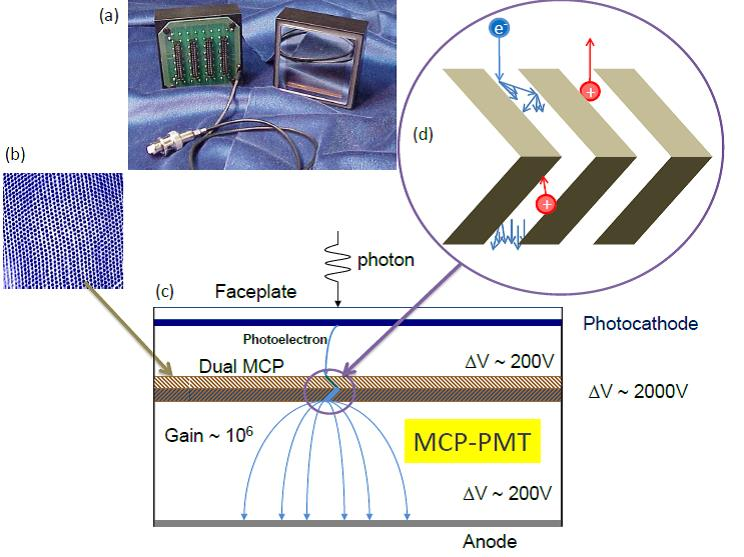
\includegraphics[width=0.45\textwidth]{images/figure1Brandt.jpg}
\caption[]{(a) a 64 channel Photonis Planacon MCP-PMT (b) an MCP (c) cartoon of the operation of an MCP-PMT (d) inset shows emission of positive ions that degrade the photocathode.}
\label{fig:PlanCon}
\end{figure}

Figure \ref{fig:PlanCon}(a) shows a photograph of a 64 channel Planacon MCP-PMT produced by Photonis \cite{Photonis}, one of the leading manufacturers of MCP-PMTs, and a strong proponent of and contributor to MCP-PMT development. Figure \ref{fig:PlanCon}(b) shows a photograph of an MCP, while Figure \ref{fig:PlanCon}(c) shows a cartoon of the MCP-PMT operation: the photo-electron is accelerated by an electric field toward a pore of the MCP in which it is multiplied, giving a typical total gain of 106; the charge is then collected on the anode giving an output pulse with a much shorter transit time ($<$1 ns) than typical PMT's as well as a narrower transit time spread (30-40 ps), resulting in excellent time resolution.   While the high voltage accelerates the electrons towards the device anode, the positive ions created from impurities in the commercial lead-silicate MCP's are accelerated back towards the photocathode (Fig. 1(d)) and eventually cause it to be irreversibly damaged, resulting in a degraded quantum efficiency (QE ). MCP-PMT lifetime is generally defined as the amount of integrated charge the phototube can absorb before its quantum efficiency (QE) degrades to 50\% of the initial value\cite{life}.  Photocathode damage is assumed to be a function of integrated charge, so high flux applications are particularly sensitive to lifetime concerns.  

\twohead{Selected Developments in Fast Timing}

Building on the success of Cherenkov-based particle ID detectors such as the BaBar experiment's DIRC detector\cite{DIRC} the Nagoya group\cite{Nagoya} took a leading role in fast timing studies for the Belle 2 Super B factory, demonstrating that a piece of quartz and an MCP-PMT could provide  $\sim$5 ps timing resolution\cite{Nagdet}. Even though this ``Nagoya'' detector did not have suitable geometry for use in an accelerator, it was vastly superior to the previous standard for time-of-flight detectors of about 100 ps \cite{TOF}, and thus contributed to a surge of interest in fast timing and MCP-PMTs.  A series of fast timing workshops mostly organized by Henry Frisch (Chicago) sprung up covering different proposed detector geometries, various photo-sensors, and fast electronics. Within the MCP-PMT community, two main groups emerged with largely orthogonal interests and approaches 1) Large Area 2) Small High Rate.  

The Large Area Picosecond Photo Detector (LAPPD)\cite{LAPPD} initiative  sought to revolutionize the MCP-PMT industry by developing a totally new large low cost ``flat panel'' 20 cm $\times$ 20 cm MCP, replacing the traditional lead glass MCP with a lower cost borosilicate option, which is less expensive and less brittle. This large group, spanning several National Labs and universities, received significant DOE funding motivated by finding a lower cost alternative to the thousands of standard phototubes required to instrument a large. LAPPD made significant progress on several fronts, but the task list proved to be long and quite challenging. Among the non-trivial challenges was replacing the lead glass flexibility and functionality with a stiffer glass such as borosilicate and developing a suitable photocathode. Abandoning lead glass MCP's requires among other things new methods of producing the array of microchannels, and new processes, for example, atomic layer deposition (ALD) to provide the emissive and resistive layers needed for the multiplication functionality. 

The second group, which pursued a more evolutionary approach, attempting to make minor modifications to existing devices was a loosely connected group comprised mainly of timing leaders from several different experiments including Mike Albrow, Jerry Va'vra, Albert Lehmann, and Brandt.

\twohead{UTA Impact on Fast Timing}

Brandt has been working on fast timing issues since 2006, initially as part of the FP420 (ATLAS/CMS) R\&D project \cite{FP420}. Although the ultimate reason for UTA's involvement was to build a fast timing system for the ATLAS Forward Proton detector, the timing detector R\&D was generic and could largely be applied to any high rate fast timing application. By late 2008, it was clear that the main challenge to building a robust 10 ps timing detector for the LHC would be the MCP-PMT rate and life time. Since Arradiance's ALD coating applied to MCP's had been demonstrated to provide excellent gain and  suppress outgassing, it seemed likely that replacing standard MCP's with these upgraded ones in an otherwise standard MCP-PMT would improve the lifetime. To speed the development,  Brandt arranged a meeting in 2009 with the principals from Arradiance and both the MCP and PMT branches of Photonis, leading  to the submission of  successful NSF Phase 1 SBIR proposal in 2011. Despite the Phase I success, Phase II was not funded primarily due to a perceived weakness in the commercialization plan.  Since then Argonne and Hamamatsu/Nagoya have been active in the ALD arena.

Over the subsequent couple of years, Arradiance and UTA worked closely with Photonis on the lifetime issue: with Arradiance applying the alumina coating to the pores of the MCP's, Photonis incorporating these modified MCP's into Planacons, and UTA testing the devices. The modified MCP's were macroscopically identical to standard ones, so could use the standard production line, avoiding some of the developmental issues that delayed LAPPD. UTA and Photonis both characterized first generation devices funded by the SBIR, and obtained lifetimes in excess of 2 C/cm$^{2}$,well-correlated to the results of gain and ion feedback measurements that Arradiance conducted prior to the ALD MCPs inclusion in the phototube. This implied that it should be possible to improve the ALD performance more economically by optimizing the external MCP performance. Idiosyncrasies in the timing distribution uncovered by UTA led to a modification of the process, resulting in the second generation ALD PMT that has been running at Erlangen for years, reaching near 10 C/cm$^{2}$ before expiring.  

\begin{figure}[htb]
\centering
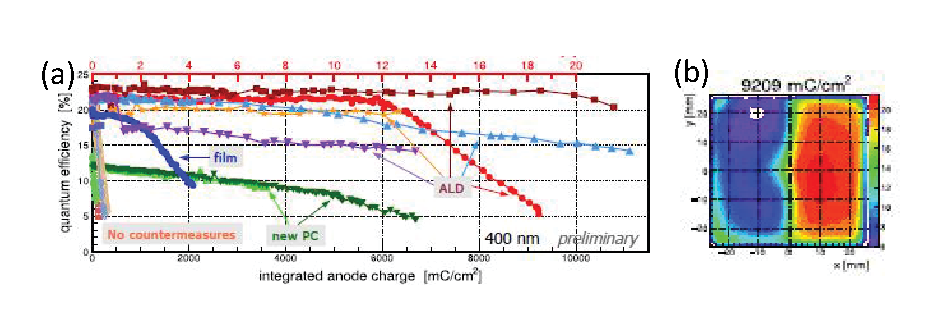
\includegraphics[width=0.85\textwidth]{images/figure2Brandt.eps}
\caption[]{(a)  Results of long term lifetime tests at Erlangen: lifetime test of 2nd generation Planacons (red) compared to the old  standard tubes (green, black, pink), a Hamamatsu ion barrier tube (blue), and a recent high vacuum tube (BINP)  (b) A half covered ALD Planacon tube indicates that the damage is mostly local.}
\label{fig:Erlangen}
\end{figure}

Figure \ref{fig:Erlangen}(a) shows an Erlangen lifetime measurement of the 2nd generation ALD Planacons (red) compared to standard tubes (green, black, pink), the Hamamatsu ion barrier tube (blue), and a new enhanced lifetime tube with a better vacuum and a more robust photocathode. (BINP). The Planacons with Arradiance ALD coating are the longest lifetime tubes in the 8 to  10  C/cm$^{2}$ range, while the Hamamatsu ion barrier tube's lifetime was a respectable, but inferior 1.8 C/cm$^{2}$, resulting in their switch to an ALD version in the middle of their production run. Their tests showed lifetimes ranging from a few to 20 C/cm$^{2}$ with a mean of about 9 C/cm$^{2}$ \cite{Nagprod}. In the last year they have made unspecified ALD improvements and claim to be on track for 20 C/cm$^{2}$.


\twohead{Work in Progress}

It has been demonstrated that by using ALD techniques one can reliably construct an extended lifetime MCP-PMT of \~10 C/cm$^{2}$ without degrading performance appreciably. While this is a tremendous accomplishment, for these devices to be a viable option for usage in very high rate environments, such as those expected for LHC experiments, it is desirable to gain a further factor of 3 or 4 to attain the target of 30 C/cm$^{2}$. Our current proposal in progress is to combine ALD technique that reduce the emission of positive ions responsible for photocathode damage with an active ion barrier that features a variable voltage mesh that can be used to repulse the positive ions that got through the ALD and keep them from reaching the photocathode. Preliminary measurements on the active ion barrier (grid tube) indicated a factor of at least 4 improvement in lifetime. 

In our ongoing  proposal (through April, 2017) we noted that we could accelerate the process by using tubes with EDR (extended dynamic range) MCP's, such that we can operate in a linear regime and obtain currents of at least 1 $\mu$ampcm$^{2}$, which would give us 1 C/cm$^{2}$  every 12 days. We also noted that if the damage is a local phenomena than we could make more than one lifetime measurement per device, which would not only be cost effective but would allow us to study the mechanism of the lifetime damage by using one tube for several measurements, one could in principle limit the systematic uncertainty due to variation in performance between devices.  We also planned to study after-pulsing rates and distributions and look for correlations between after-pulsing and lifetime.  We proposed to use new mini-planacons (these 1 in $\times$ 1 in,tubes are basically one-fourth of a planacon)  for the studies, since they were less expensive and our budget is modest. 

\begin{figure}[htb]
\centering
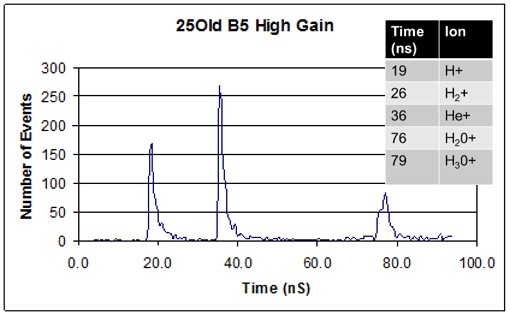
\includegraphics[width=0.55\textwidth]{images/figure3Brandt.jpg}
\caption[]{Ion feedback measurement in a Planacon.}
\label{fig:ionfeedback}
\end{figure}

Based on our experience and new developments we have modified our program somewhat. We determined that the mini-planacon is not suitable for the studies, as it is too small to make multiple independent measurements. We determined that one has to be very rigorous with the pre-lifetime tests as it is prudent to tune the front and backstage voltage, which affect collection efficiency and shower size, respectively. This is necessary since the ALD tubes have an intrinsically higher gain, and consequently require less high voltage across the MCP, with a fixed voltage divider this results in less high voltage across the front and back stage as well, so we developed variable voltage dividers. Figure \ref{fig:ionfeedback} shows a representative after pulsing measurement. We found that some  after pulsing measurements were subject to subtle noise effects that were not evident in other measurements due to relatively low rates and small time windows, became relevant for the long lifetime tubes.  Finally, with the LAPPD R$\&$D effort winding down, DOE is interested in seeing life time measurements of the Incom, and Argonne devices (see Appendix 9). 

\twohead{Proposed Research and Methods}

Building on a successful R\&D effort that has seen the MCP-PMT  lifetime increase by a factor of 50 from 0.2 to 10 C/cm2  our goal is to demonstrate a life time of 30 C/cm$^{2}$. This goal is supported by the following objectives.1)Assess the viability of multiple measurements per device. If it can be demonstrated that one could get several consistent measurements from the same tube this would not only reduce cost, but reduce systematic uncertainty that stems from tube to tube variation. 2) Determine if the method of damage to the tube is correlated to the lifetime by comparing the life time under different aging conditions.  Is high rate low gain equivalent to low rate high gain?  Is a blue pulsed LED equivalent to a continuous white light source? 3) Set up a dedicated test station where several tubes can be simultaneously measured. 4) Determine whether the overall after pulsing rate or a subset of it is correlated with lifetime 5) Characterize and life test LAPPD MCP-PMTs.

\twohead{Work Plan}

The group that will carry out the project work consist of the PI, a post-doc working half time on the project, an early career graduate student and two undergraduates. We have been trying to operate without a post-doc, but there is a lot of details and subtleties to the issues, and the absence of mid-level management has slowed progress.  These tests will be carried out at the UTA Picosecond Test Facility (PTF) in the Chemistry and Physics Research building.  The PTF was established using funds from the Texas Advanced Research Program and the Department of Energy Advanced Detector Research program.  The main components are a light-tight box containing a Hamamatsu PLP-10 pulsed picoseconds laser, with 405 and 635 nm laser diode heads, various associated optical equipment (lenses, mirrors, beam splitters, and filters), electronics including a precision programmable CAEN N1470 high voltage unit, specialized fast amplifier circuit boards with low noise mini-circuit amplifiers and programmable attenuators, precision constant fraction discriminators (<5 ps resolution),  and two fast scopes a LeCroy 6 GHz Wavemaster 8620A and a LeCroy 6 GHz, 40 Gs/s 760zi-a WavePro oscilloscope.   The amplifiers and CFDs were developed by Stony Brook with a sub-award from Brandt's second DOE ADR grant. 

The students will carefully pre-test each tube before lifetime testing it in order to establish a performance baseline. This includes the initial amplitude, gain, transit time, after pulsing rate, etc. We will use the 6 GHz LeCroy 8620 Wavemaster scope to monitor the pulse amplitude, number of photoelectrons, and time resolution. We have written automatic scripts that take data once/hr, then the scope sleeps for 55 minutes and repeats the cycle.  

The ability to do multiple measurements with one device is an important element in the plan, and must be resolved before we can life test the unique tubes. The pixel-based life time approach assumes that the lifetime damage is essentially a local phenomenon. Figure 2(b) showed the damage to a tube where the left half was exposed and the right half was not.  It appears that the damage is a local effect, but since a tube is good until it starts going bad, this is not definitive. We will do a definitive test  with an old 4 channel Planacon and sequentially expose one quadrant while monitoring all four.  Ideally the 4 measurements are consistent, or at least follow a reproducible trend. We can apply a similar approach with an old 64 channel tube, taking  3$\times$3 pixel regions in each of the four corners of the tub and illuminating the central pixel, for example,  pixels (2,2),  (2,7), (7,2), (7,7). This would leave a buffer of the central two rows and columns between the four quadrants, in principal isolating them.  One could then apply the light source to the above cells or one of the nine cell grids. Four independent measurements per tube would be very useful.   

There are two main modes of operation that require long life tubes, the LHC mode has high rate (several MHz), 10 pe's, and a moderate gain of about 1x105  while the Panda approach has high rate, 1 pe, and high gain (1x106). Although both tests cannot be done simultaneously, it is important to cross check the lifetime with each approach, to verify that the new tube will be suitable for both modes of operation. A different quadrant would be used for the ``PANDA'' test after the ``LHC'' test is complete.   With the special low resistance versions of the tubes, we can obtain currents in excess of 1 A/cm$^{2}$ or more, corresponding to a Coulomb/cm$^{2}$ of charge every 12 days. The more extreme second approach to accelerating the lifetime measurement is to run the tube in a partially saturated mode, the realm where the current is no longer increasing linearly with laser repetition rate. We can investigate our expectation that the lifetime scales with the extracted charge and not the input charge from the number of incident photons. 

The next step is to develop a dedicated lifetime test stand capable of accelerated testing of multiple tubes.With the current grant we have purchased most of the necessary components that we could not scrounge: the light source (LED, laser), optical equipment (lens, mirrors, filters), the phototubes being tested and associated tube holders, a few cables, amplifiers and their associated low voltage, high voltage for the MCP-PMT, fibers to distribute the light, etc. Tests have typically been  performed using  the PLP-10 laser, which has variable repetition rate from 1 Hz to 100 MHz, with neutral density filters used to control the amount of light incident on the tube.  We are adding a pulsed LED setup in a second light tight box, allowing for multiple simultaneous lifetime tests to be carried out.  The establishment of a dedicated lifetime component of the PTF is essential as the lifetime of the tubes increase, and for systematic studies, and allows the standard setup to be used in parallel for characterization.

When the preliminaries are finished we will test four tubes to pin down the lifetime correlations. Photonis is providing three custom tubes at a deep discount: an ALD tube, a grid tube, and the combined ALD-grid tube. The fourth MCP-PMT which we have in-hand will be a standard Photonis tube to serve as a control.
 
The final work plan includes testing the LAPPD tubes, which are anticipated to have long lifetime due to the use of an alternate glass from lead glass, but have not been lifetime tested. This is beyond the scope of Argonne's MCP operations, and also INCOM does not have this capability in house. 

\twohead{Resources required}
This proposal heavily leverages previous investment by the Department of Energy in Professor Brandt and his Picosecond Test Facility, and the LAPPD collaboration. Most of the equipment resources needed for this proposal are already part of the Picosecond Test Facility. 
The new Photonis tubes are paid for and should be delivered by the end of 2017.   The LAPPD group will provide us their device(s) in exchange for testing.  The only cost is personnel, one month of summer salary each year for the PI, and 50\% of a post-doc the first two years to help complete the dedicated lifetime station, and supervise locally financed undergraduate students who will be performing some of the tests. The post-doc will help oversee the test stand construction, and help interface the test stand with the LAPPD devices. In the third year, we do not anticipate development, but rather fairly routine testing, so two undergraduates are expected to be capable of finishing the work associated with this proposal timeline of tasks is as follows.

\twohead{Timeline}

From now until March we will validate the quadrant-based lifetime approach with an existing device and debut our accelerated testing with second quadrant tube. 4/1/17-9/30/17 pretest 3 Photonis custom tubes, (tune front and backstage voltage), life test of the custom tubes.10/1/17-3/31/18 Evaluate Argonne tube with laser, figure out how to use striplines? 4/1/18-9/30/18 Lifetime of $20 \times 20$ evaluate a traditional (no stripline) $6\times 6$  10/1/18-3/31/19 finish with LAPPD testing 4/1/19-3/31/20 additional life tests and other measurements as needed. 

The technical and intellectual merits of this proposal are noteworthy.  The life time has been extended by a factor of about 50 in the last 5 years.  Further lifetime improvement will be attempted through the optimization of nanofilm combined with the active ion barrier. UTA and Arradiance Inc. have developed techniques to study ion generation both in the MCP test stand and in situ examination of the MCP-PMT after-pulsing which correlated to lifetime can determine the root cause of lifetime degradation. The LAPPD devices are nearing completion and could have excellent lifetime and find a niche in the market.

The broader impacts of this proposal are substantial. Image intensification detection devices incorporating MCP's are currently widely used in applications where single photon counting or low light level detection is required, but cannot be used in high rate environments. Super-Belle II and Panda are evaluating the use of MCP-PMTs, and the long-life device could easily become a staple of HEP experiments. The impact of an improved lifetime device extends beyond cutting edge particle physics experiments as detectors with exciting discovery potential in the areas of CP violation and Higgs properties, to homeland security and night vision applications.  The testing of the new MCP-PMT's will continue to be partially carried out by undergraduate students at UTA, which ranks in the top 15 in the country in student diversity.  This proposal thus supports the specific mission of DOE for the HEP community and leads to great research opportunities for undergraduates.
